\documentclass{article}
\usepackage[utf8]{inputenc}
\usepackage{datetime}
\usepackage{enumerate}
\usepackage{textcomp}
\usepackage{amsmath}
\usepackage{amssymb}
\usepackage[edges]{forest}
\usepackage{tikz}
\usetikzlibrary{shapes, backgrounds, automata, positioning, arrows}
\usetikzlibrary{arrows}
\usepackage{listings}
\usetikzlibrary{graphs}

\usepackage{titlesec}
\newcommand{\sectionbreak}{\clearpage}
\def\math#1{$#1$}

\title{HW4}
\author{Xinhao Luo}
\date{\today}

\begin{document}

\maketitle

\section{DPV  Problem  5.15}
\begin{enumerate}[a)]
    \item Possible frequency example: $f_a = 0.5$, $f_b = 0.25$, $f_c = 0.25$
    \item Not possible: only leaf nodes should be used to encode 
    \item Not Possible: It cannot form a full binary tree
    \item Code: \{0, 100, 1010, 1011, 11\} \\
         Possible frequency example: $f_a = 0.5$, $f_b = 0.25$, $f_c = 0.125$, $f_d = 0.0625$, $f_e = 0.0625$
\end{enumerate}
  
\section{DPV Problem 5.16}
\begin{enumerate}[a)]
    \item Prove by contradiction
        \begin{itemize}
            \item Assume there is no codeword of length 1
            \item If there is a no codeword of length 1, the minimum tree we have should like this: \\\\
            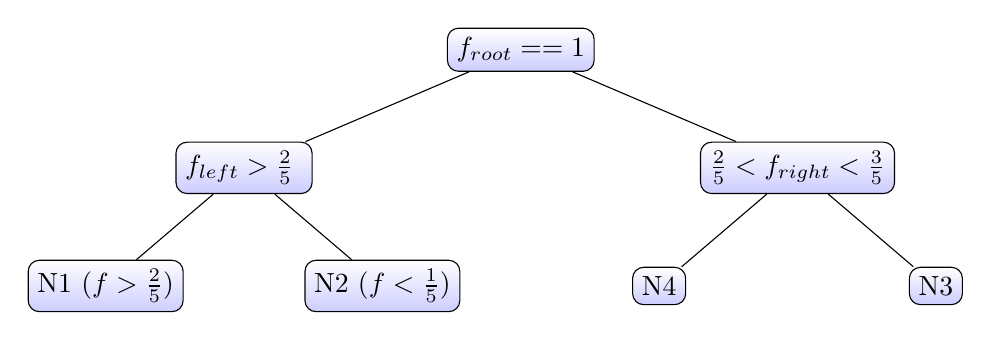
\begin{tikzpicture}[sibling distance=10em,
              every node/.style = {shape=rectangle, rounded corners,
                draw, align=center,
                top color=white, bottom color=blue!20}]]
              \node {\math{f_{root} == 1}}
                child { node { \math{f_{left} > \frac{2}{5}} } 
                        child { 
                            node {N1 (\math{f > \frac{2}{5}})} 
                        }
                        child { node {N2 (\math{f < \frac{1}{5}})} }
                }
                child [missing]
                child { 
                    node {\math{\frac{2}{5} < f_{right} < \frac{3}{5}}}
                    child {node {N4}}
                    child {node {N3}}
                };
            \end{tikzpicture}
            \item Assume N1 is the node with more than \math{\frac{2}{5}} frequency, then its parent would also larger than \math{\frac{2}{5}} as it is the sum of its children.
            \item On the other half of the tree, we may have in total \math{\frac{2}{5} < f < \frac{3}{5}} since we need to ensure \math{f_{root} == 1}
            \item However, if the other half of the tree has already larger than \math{\frac{2}{5}}, and its neighbour, at the same time, occupy at least \math{\frac{2}{5}}, N2 must be \math{f < (1 - \frac{2}{5} - \frac{2}{5} = \frac{1}{5})}
            \item At the same time, the biggest frequency N3, N4 can get is \math{\frac{3}{5} \times \frac{1}{2} = \frac{3}{10}}, which is smaller than N1
            \item The rules defined that each time, two smallest nodes will be combined. N2 should be bind with either N3, N4 rather than N1, which is fishy
            \item This graph does not exist and the assumption is false
    \end{itemize}
    \item Prove by contradiction
        \begin{itemize}
            \item Assume there is codeword of length 1
            \item If there is a no codeword of length 1, the minimum tree we have should like this: \\\\
            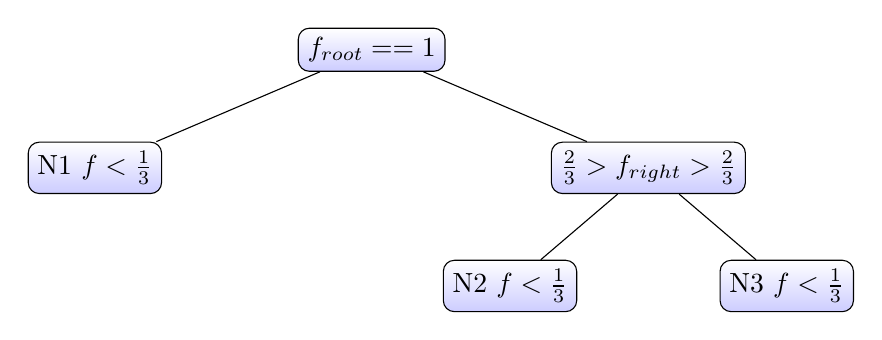
\begin{tikzpicture}[sibling distance=10em,
              every node/.style = {shape=rectangle, rounded corners,
                draw, align=center,
                top color=white, bottom color=blue!20}]]
              \node {\math{f_{root} == 1}}
                child { node {N1 \math{f < \frac{1}{3}}}}
                child [missing]
                child { 
                    node { \math{\frac{2}{3} > f_{right} > \frac{2}{3}}}
                    child {node {N2 \math{f < \frac{1}{3}}}}
                    child {node {N3 \math{f < \frac{1}{3}}}}
                };
            \end{tikzpicture}
            \item Assume N1 is the node with codelength 1, then the other half of the tree will be \math{f_{right} > \frac{2}{3}}
            \item However, since each leaf can only be \math{\frac{1}{3}}, we will also have \math{f_{right} < \frac{2}{3}}
            \item \math{f_{right}} does not exist, so the graph does not exist, which means the assumption is false
        \end{itemize}
\end{enumerate}

\section{DPV Problem 2.17} 

General idea: Doing binary search over the array \\

\textbf{Algorithm}

Assume index start from 1

\begin{enumerate}[Step 1]
    \item Take the length of A as \math{l}
    \item Take \math{half = l} // 2
    \item Compare \math{half} and \math{A[half]}
        \begin{itemize}
            \item If \math{half > A[half]}, start from step 1 with \math{A = A[1:(half - 1)]}
            \item If \math{half < A[half]}, start from step 1 with \math{A = A[(half + 1):l]}
            \item If \math{half == A[half]}, return \math{half}
        \end{itemize}
\end{enumerate}

\textbf{Runtime} \\

Using master theorem, we have: \math{T(n) = 1 * T(n/2) + O(1)}

\begin{itemize}
    \item The merge part does nothing, so we have \math{O(1)}, \math{1 = n^0}, so \math{d = 0}
    \item Each time, we have split the array into half and discard one of them, so we have \math{b = 2}
    \item In each iteration, we only start over once, so \math{a = 1}
\end{itemize}

\begin{itemize}
    \item \math{a = 1}, \math{b = 2}, \math{log_ba = log_21 = 0}
    \item \math{d = 0 = log_ba}, so we have \math{O(n) = n^dlogn = n^0logn = logn}
\end{itemize}



\section{DPV Problem 2.19} 
\begin{enumerate}[a)]
    \item \begin{equation}
        \begin{split}
            T(k, n) &= O(n, n) + O(2n, n) + ... + O((k - 1)n, n) \\
            &= O(2n + 3n + ... + kn) \\
            &= O(n \times \sum_{i = 2}^ki) \\
            &= O(n\frac{(2 + k)(k - 1)}{2}) \\ %约成k^2
            &= O(k^2n)
        \end{split}
    \end{equation}
    \item \textbf{Algorithm}
        Define \math{merge(a1, a2)} that takes two sorted array and return one sorted array. The whole process should take \math{O(2n) = O(n)}
         \begin{verbatim}
            def sort(arrays):
                if len(arrays) < 2:
                    return arrays[0]
                elif len(arrays) < 3:
                    return merge(array[0], array[1])
                else:
                    size = (len(arrays) - 1) // 2
                    return merge(sort(arrays[0:size]), sort(arrays[size:]))
         \end{verbatim}
    \textbf{Runtime}
    Using master theorem, we have: \\ 
        \math{T(kn) = 2 * T(k/2) + O(kn)} \\
        \math{T(k) = O(1)} when \math{n = 1}
    \begin{itemize}
        \item The merging process will take \math{O(kn^1)} as it will need to go through each element once. \math{d = 1}
        \item Each time, the method will recur twice, \math{a = 2}
        \item Each time, the length of the array is cut by half, \math{b = 2}
        \item \math{log_ba = log_22 = 1 = d}, 
        \item \math{T = O(knlog{n})}
    \end{itemize}
\end{enumerate}

\section{DPV Problem 2.23}
\begin{enumerate}[a)]
    \item 
        \textbf{Algorithm} Takes two a, b as parameters
        \begin{enumerate}
            \item Recursively split the array into half and look for each sublist's majority, and merge two sublist's result
            \item If two sublist has the same majority, then return the majority
            \item If two sublist has different majority, go through the merged array and find these two majority's frequency and compare
            \item If one sublist has a majority while the other don't have, count if this element is the majority after merged
            \item If two sublist both don't have the majority, no majority appears
        \end{enumerate}
        \textbf{Runtime} 
        \begin{enumerate}
            \item Based on master's theorem, we may have \math{T(n) = 2 \times T(n/2) + O(n)}
            \item each time, we called ourselves twice, cut the list by half, and each time we need to count the elements on necessary
            \item \math{a = 2, b = 2, d = 1}, \math{log_ba = log_22 = 1 = d}
            \item \math{O(n) = nlogn}
        \end{enumerate}
    \item 
        \textbf{Algorithm} Takes an array of elements
        \begin{enumerate}[Step 1]
            \item Split the array into pairs, we now have \math{n / 2} pairs
            \item for each pairs, discard if the pairs are not the same, else keep one of the elements in the pair. Now we at most will have \math{n_{new} \leq n_{old} / 2} elements
            \item Return to step 1 if more than 1 elements remains
            \item If there is one elements left, this element will be the majority, otherwise no majority
            \item If there is odd number of element appears, get its frequency after pairs, if it is the majority, return that element, or discard it
        \end{enumerate}
        \textbf{Runtime} 
        \begin{enumerate}
            \item Based on master's theorem, we may have \math{T(n) = 1 \times T(n/2) + O(n)}
            \item each time, we called ourselves once each time; cut the list by half, and each time we need to compare the result at the end
            \item if there is odd number of element, after \math{O(n)} pairs, then do an \math{O(n)} search. \math{O(2n) = O(n)}
            \item \math{a = 1, b = 2, d = 1}, \math{log_ba = log_12 = 0 < d}
            \item \math{O(n) = n}
        \end{enumerate}
\end{enumerate}

\end{document}
